\chapter{Using a Nexys4DDR as a MEGA65}

\section{Building your own MEGA65 Compatible Computer}

You can build your own MEGA65-compatible computer by using a Nexys4DDR (Nexys A7) FPGA development board.
This appendix describes the process to setup a Nexys4DDR board for this purpose.
The older non-DDR Nexys4 board is also supported, and the instructions are the same, except that
you must use a bitstream designed for that board.
Using a Nexys4DDR bitstream on a non-DDR Nexys4 board, or vice versa, may cause irreparable damage to your board, so make sure
you have the correct bitstream to suit your board.


DISCLAIMER: M.E.G.A cannot take any responsibility for any damage that may occur to your Nexys4DDR board.

\newpage

\section{Power, Jumpers, Switches and Buttons}

The Nexys4DDR board can be powered in two ways: using an external power supply, or from a standard USB port.

\subsection{Micro-USB Power}

\includegraphics[width=5cm]{images/illustrations/nexys-micro-usb-power.pdf}

Connect your micro-usb cable to a USB port on a USB charger or PC to provide power. Connect the other end to the Nexys4DDR's micro-usb connector. Place the JP3 jumper on pins 1 and 2 to select USB power. Use the switch to turn on the Nexys4DDR.

\subsection{External Power Supply}

\hspace*{1.7cm}
\includegraphics[width=3.2cm]{images/illustrations/nexys-power-supply.pdf}

The MEGA65 core can consume a lot of power, and a standard USB port could potentionally be too little for the Nexys4DDR board. In particular, writing to the SD card might hang or perform odd behaviour. Therefore you should consider a 5V power supply.

Digilent sell a power supply for the Nexys4DDR board, and we recommend you use this to ensure you avoid the risk of damage to your Nexys4DDR board. The chosen power supply should be center positive, 2.1mm internal diameter plug, and should deliver 4.5VDC to 5.5VDC rated at least 1 Amp.

Connect the power supply cable to the supply plug of the Nexys4DDR. Place the JP3 jumper on pins 2 and 3 to select WALL power. Use the switch to turn on the Nexys4DDR.

\subsection{Other Jumpers and Switches}

Set the following jumpers on your Nexys4DDR board to the following positions:

\begin{itemize}
\item{JP1} - USB/SD
\item{JP2} - SD
\end{itemize}

% XXX - Image of board highlighting the jumpers

All 16 switches on the lower edge of the board must be set to the off position.


\subsection{Connections and Peripherals}

\includegraphics[width=\linewidth]{images/illustrations/nexys-connectors.pdf}

A USB keyboard can be connected to the USB port. Only a keyboard that lacks a USB hub will work with the Nexys4DDR board.  Generally extremely cheap keyboards will work, while more expensive keyboards tend to have a USB hub integrated, and will not work.  You may need to try several keyboards, before you find one that works.

You can connect a VGA monitor to the VGA port.

The mono audio-out jack can be connected to the line-in of an amplifier.

\subsection{Onboard buttons}

\begin{center}
  \includegraphics[width=3.2cm]{images/illustrations/nexys-reset-buttons.pdf}
\end{center}

The ``CPU RESET'' button will reset the MEGA65 when pressed, while the ``PROG'' button will cause the FPGA itself to reload the MEGA65
core.  The main difference between the two is that CPU RESET is faster, and does not clear the contents of memory, while the FPGA button
is slower, and does reset the contents of memory.

\begin{center}
  \includegraphics[width=3.2cm]{images/illustrations/nexys-five-buttons.pdf}
\end{center}

Two of the five buttons in the cross arrangement can also be used:  BTND acts as though you have pressed the \megakey{RESTORE} key, while BTNC will trigger an IRQ, as though the IRQ line had been pulled to ground.

\section{Keyboard}

The keyboard layout is positional rather than logical.
This means that keys in similar positions to the keys on a C65 keyboard will have similar function.
This relationship assumes that your USB keyboard uses a US keyboard layout.

To help you locate what the various MEGA65 keys are mapped to, the MEGA65 has a built-in virtual keyboard test feature. This can be accessed in two ways.

The easiest way is to keep the \specialkey{ALT} key held in while turning on the Nexyx4, or resetting the Nexyx4 with the ``PROG'' button. The configure menu will be presented and by pressing 3, the virtual keyboard will be presented on a black background.

\includegraphics[width=\linewidth]{images/illustrations/virtual-keyboard.pdf}

Pressing a key on the USB keyboard will show the highlighted key on the virtual keyboard to help you identify the key mapping.

The other way to access the virtual keyboard is from within the MEGA65. Hold \megasymbolkey and press \megakey{TAB} to access the Matrix Mode Debugger. From here, enter the following:

\screentextwide{s ffd3615 ff}

This will open a semi-transparent virtual keyboard at the top of the screen. Alternatively:

\screentextwide{s ffd3615 ff ff}

This will open a semi-transparent virtual keyboard in the centre of the screen.

Hold \megasymbolkey and press \megakey{TAB} to exit Matrix Mode Debugger and return to the MEGA65.

\subsection{Some key mappings with a USB keyboard}

The \megakey{RESTORE} key is mapped to the PAGE UP key.

The \specialkey{RUN STOP}  key is mapped to the ESC key.

\newpage

\section{Preparing microSDHC card}

The MEGA65 requires an SDHC card of between 4GB and 64GB capacity.  Some SDXC cards may work, however, this is not officially supported.

To prepare your SD card, you will need the following files from the MEGA65 Filehost:

\subsection{Bitstream File}

Visit the following url:

\url{https://mega.scryptos.com/sharefolder-link/MEGA/MEGA65+filehost/Bitstreams/Jenkins-Out/mega65-core/development/}

Sort the list of build folders by 'Date' and click on the latest:

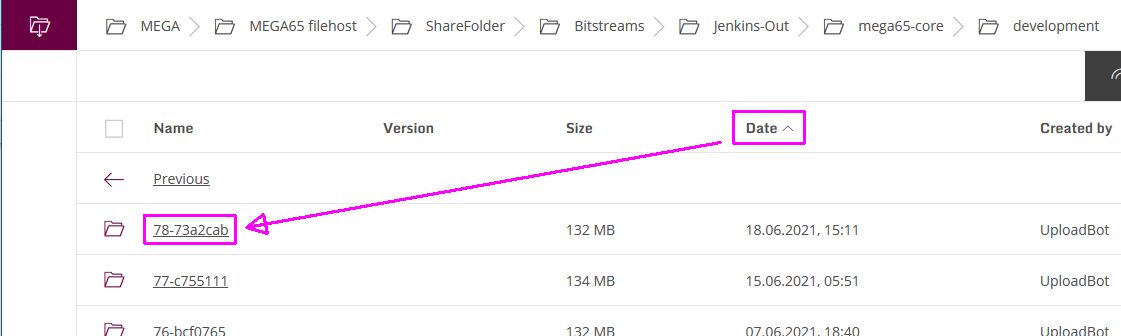
\includegraphics[width=\linewidth]{images/latest_bitstream.png}

Download either:

\begin{itemize}
  \item{\textbf{nexys4.bit} (for Nexys4 PSRAM boards)}
  \item{\textbf{nexys4dd4-widget.bit} (for Nexys4 DDR boards)}
  \item{You can also find bitstream files for various other m65 targets here (mega65r2, mega65r3)}
  \item{You can also find core (.cor) files located here (See \nameref{cha:cores} chapter for more details on how to make use of them)}
\end{itemize}

\subsection{Support Files}

For official owners of the MEGA65 (both devkit and final product), visit the following url and log in with the user credentials you have been provided. This will take you to the MEGA65 Filehost location where the "\textbf{MEGA65 SD card essentials}" download page is located. Then click the "\textbf{Download}" link to retrieve the latest "\textbf{SD essentials.rar}" file. 

\url{https://files.mega65.org?id=a809e0ae-30ac-42f5-ab9c-766d72fd6331}

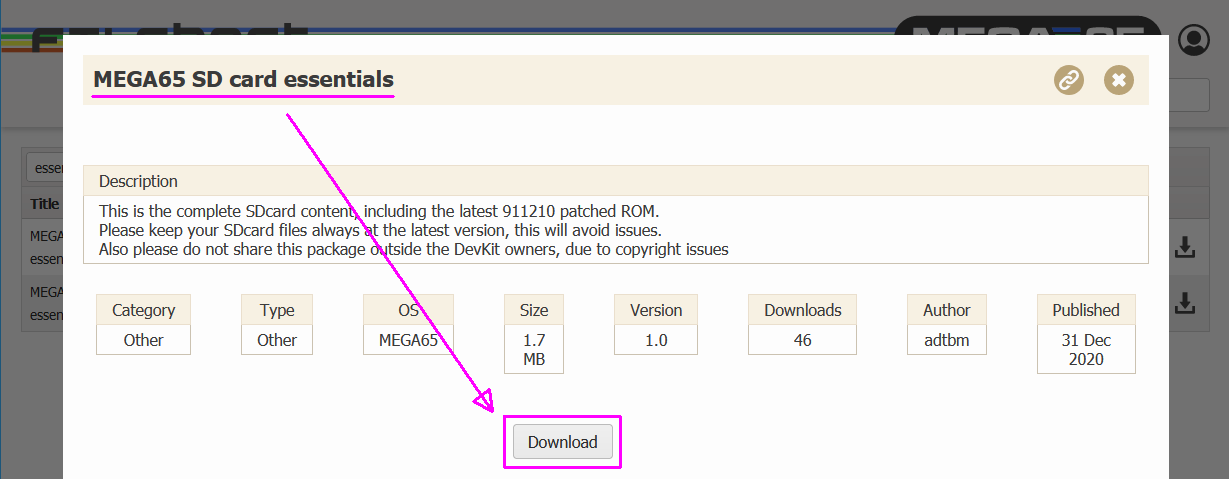
\includegraphics[width=\linewidth]{images/latest_support_files_with_closedrom.png}

Note that this link is only available to official owners of the MEGA65 product, as the fileset also contains the licensed closed-source MEGA65.ROM file.

For Nexys board owners in search of a similar fileset (without the ROM), visit the following url instead:

\url{https://files.mega65.org/?id=0fb941fe-5c5f-4608-b0f1-32849d4a8dff}

This will take you to the MEGA65 Filehost location where the "\textbf{MEGA65 SD card essentials - No ROM}" download page is located. Click the "\textbf{Download}" link to retrieve the latest "\textbf{SD essentialsNoROM.rar}" file.

Note that while this fileset does not contain a ROM, there are future plans for it to include the freely available OpenROM.

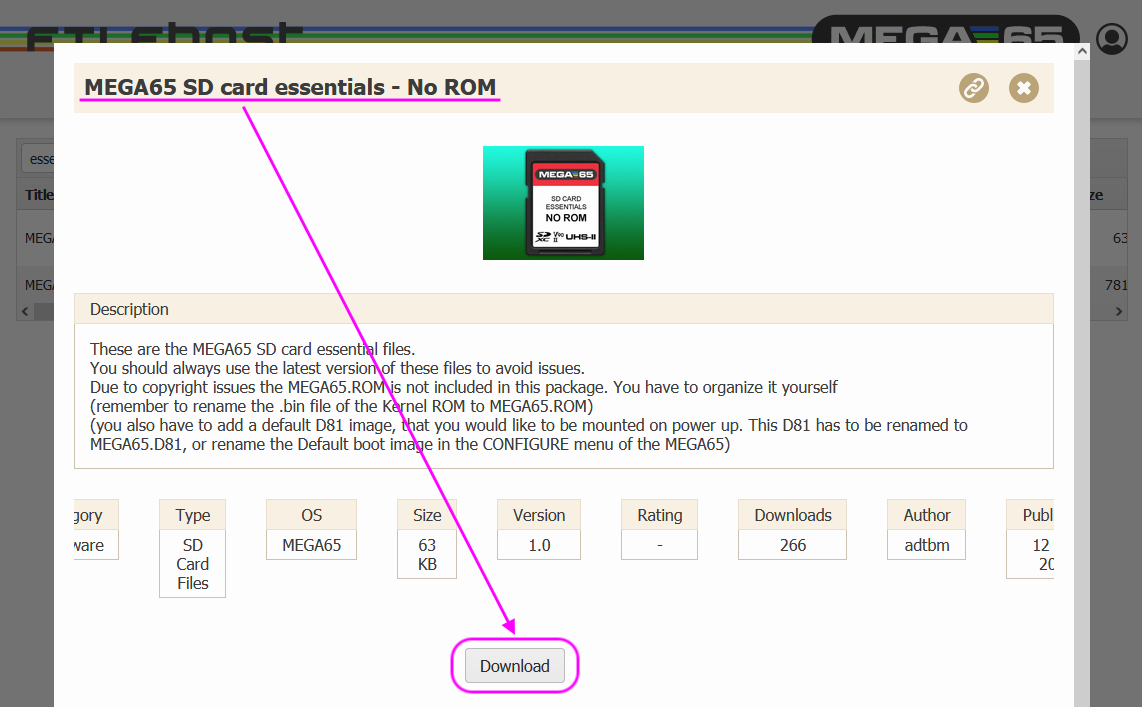
\includegraphics[width=\linewidth]{images/latest_support_files.png}

\subsection{ROM File}

\textbf{Original C65 ROMs}

You may want to source your own separate C65 ROM via other means.  There were many different versions created during the development of the Commodore 65,
and the MEGA65 can use any of them.  However, out of this set, we recommend you use 911001.bin, as this has the most complete BASIC and DOS implementations.

\textbf{MEGA65 ROMs}

There are newer versions of the \textbf{MEGA65 Closed ROM} actively under development also. These ROMs improve upon the original C65 ROMs and make better use of the extra hardware capabilities that the MEGA65 has over the original C65 hardware. These ROMs are available via the filehost also, but only to owners of the MEGA65, who will need to log into the filehost with their credentials in order to download it. It can be located by visiting the "\textbf{Files}" tab and searching for "\textbf{kernel rom}":

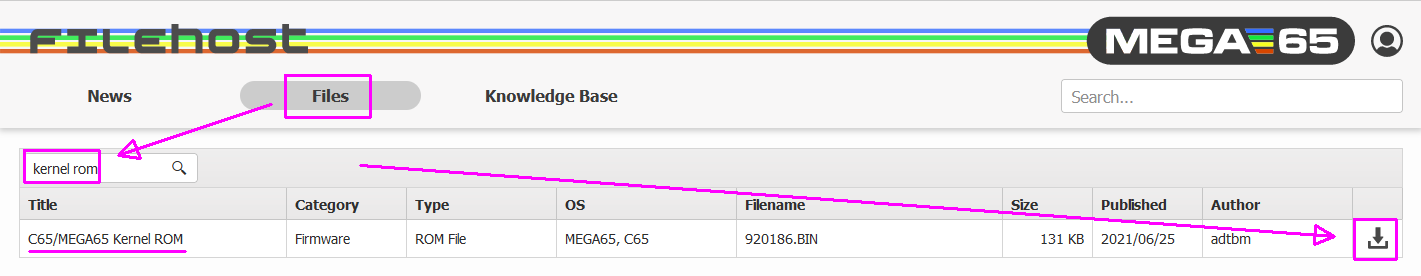
\includegraphics[width=\linewidth]{images/latest_closed_rom.png}

\textbf{MEGA65 ROM diff files}

If you have sourced your own 911001.bin C65 ROM and would like to patch it to the latest MEGA65 ROM, we do provide patches, as the additional improvements we have made to the closed rom are open source. Those diff files are available here:

\url{https://files.mega65.org?id=fd2c40b9-f337-41f7-8a81-0254b1e09fb5}

\textbf{MEGA65 OpenROMs}

Another available option is to make use of \textbf{MEGA65 OpenROMs}. The latest version of this is always downloadable from either of the following urls:

\begin{itemize}
  \item \url{https://files.mega65.org?id=8aec2fba-3b0a-4677-80ae-7a7f5f4f0cb8}
  \item \url{https://github.com/MEGA65/open-roms/raw/master/bin/mega65.rom}
\end{itemize}

\subsection{Preparation Steps}

The steps are:

\begin{itemize}
  \item{Format the SD card} in a convenient computer using the FAT32 file-system.  The MEGA65 and Nexys4DDR boards do not understand other
file systems, especially the exFAT file system.
\item{Copy} your bitstream file (with name ending in ``.bit'') onto the SD card.
\item{Insert} the SD card into the SD card slot on the under-side of the Nexys4DDR board.
\item{Turn on} the Nexys4DDR board.
\item{Enter the Utility Menu} by holding the \megakey{ALT} key down on the USB keyboard you have connected to the Nexys4DDR board.
\item{Enter the FDISK/FORMAT tool} by pressing 2 when the option appears on the MEGA65 boot screen.
\item{Follow the prompts} in the FDISK/FORMAT program to again format the SD card for use by the MEGA65. \\
  \\
  The FDISK tool will partition your SD card into two partitions and format them.
  \begin{itemize}
    \item One is type \$41 = MEGA65 System Partition, where the save slots, configuration data and other files live. \\
  (This partition is invisible in i.e. Win PCs).
    \item The other partition with type \$0C = VFAT32, where KERNEL, support files, games, and so on, will be copied to later. \\
  (This partition is visible on i.e. Win PCs).
  \end{itemize}
\item{Once formatting is complete}, switch off the Nexys4DDR board and remove the microSDHC card from the Nexys board and put it back into your PC
\item{This time, copy} the following items onto the SD card:
  \begin{itemize}
    \item The bitstream file
    \item The extracted files from within either the "\textbf{SD essentials.rar}" or "\textbf{SD essentialsNoROM.rar}" file that you downloaded from the MEGA65 filehost.
    \item{If you have sourced your own preferred ROM file} (e.g. "\textbf{911001.BIN}"), copy it onto the SD card also, and rename it to "\textbf{MEGA65.ROM}" (uppercase is essential).
    \item{Any .D81 disk image files} you wish to make use of.
      \begin{itemize}
        \item Note that if a file named MEGA65.D81 is added to the SD card, it will be mounted automatically on startup.
        \item Make sure that all .D81 files have names that fit the old DOS 8.3 character limit, and are upper case.  This restriction will be removed in a future release.
      \end{itemize}
  \end{itemize}
\item{Remove the SD card} and reinsert it into your Nexys4DDR board.
\item{Power the Nexys4DDR} board back on.  The MEGA65 should boot within 15 seconds.
\end{itemize}

\quote{Congratulations. Your MEGA65 has been set up and is ready to use.}

Please note that the above method of copying the bitstream file to the SD card means that the bitstream is loaded into the Nexys FPGA each time on boot - which takes around 13 seconds for the system to start. The bitstream can also be flashed using Vivado software into the QSPI flash to deliver a boot up time of 0.3 seconds.  

For more detailed information on preparing and configuring your MEGA65, please refer to the \nameref{cha:configuring} chapter. 

\section{Useful Tips}

The following are some useful tips for getting familiar with the MEGA65:

\begin{itemize}

\item{Press \& hold \megasymbolkey (or the Commodore key if using a Commodore 64 or 65 keyboard) during boot to start up in C64 mode instead of C65 mode}
 \item{Press \& hold \specialkey{RUN STOP} during boot to enter the machine language monitor, instead of starting BASIC.}
\item{Press the \megakey{RESTORE} key for approximately 1/2 - 1 second to enter the MEGA65 Freeze Menu.  From this menu
  you have convenient tools to change the CPU speed, switch between PAL \& NTSC video mode, change Audio settings, manage freeze-states,
   select D81 disk images, examine and modify memory of the frozen program, among other features.  This is in many ways the heart of the MEGA65, so it is well worth exploring and getting familiar with.}
\item{Type \screentext{POKE0,65} in C64 mode to switch  the CPU to full speed (40MHz). Some software may behave incorrectly in this mode, while other software will work very well, and run many times faster than on a C64.}
\item{Type \screentext{POKE0,64} in C64 mode to switch the CPU to 1MHz.}
\item{Type \screentext{SYS58552} in C64 mode to switch to C65 mode.}
\item{Type \screentext{GO64} in C65 mode and confirm, by pressing \screentext{Y}, to switch to C64 mode, just like on a C128.}
\item{The C65 ROM makes device 8 the default, so you can normally leave off the \textbf{,8} from the end of LOAD and SAVE commands.}
\item{Pressing \megakey{SHIFT} + \specialkey{RUN STOP} from either C64 or C65 mode will attempt to boot from disk.}
\end{itemize}

Have fun! The MEGA65 has been lovingly crafted over many years for your enjoyment. We hope you have as much fun using it as we have had creating it!

The MEGA Museum of Electronic Games \& Art welcomes your feedback, suggestions and contributions to this open-source digital heritage preservation project.
